\documentclass[paper=letter, fontsize=11pt]{scrartcl} % A4 paper and 11pt font size
\synctex=1
\usepackage[T1]{fontenc} % Use 8-bit encoding that has 256 glyphs
\usepackage{fourier} % Use the Adobe Utopia font for the document - comment this line to return to the LaTeX default
\usepackage[english]{babel} % English language/hyphenation
\usepackage{amsmath,amsfonts,amsthm} % Math packages
%\usepackage[nolists, nomarkers]{endfloat}
\usepackage{hyperref}
\usepackage{bm}
\usepackage{graphicx}
\usepackage[section]{placeins}
\usepackage{sectsty} % Allows customizing section commands
\allsectionsfont{\normalfont\scshape} % Make all sections centered, the default font and small caps

\usepackage{fancyhdr} % Custom headers and footers
\pagestyle{fancyplain} % Makes all pages in the document conform to the custom headers and footers
\fancyhead{} % No page header - if you want one, create it in the same way as the footers below
\fancyfoot[L]{} % Empty left footer
\fancyfoot[C]{} % Empty center footer
\fancyfoot[R]{\thepage} % Page numbering for right footer
\renewcommand{\headrulewidth}{0pt} % Remove header underlines
\renewcommand{\footrulewidth}{0pt} % Remove footer underlines
\setlength{\headheight}{13.6pt} % Customize the height of the header

% \numberwithin{equation}{section} % Number equations within sections (i.e. 1.1, 1.2, 2.1, 2.2 instead of 1, 2, 3, 4)
% \numberwithin{figure}{section} % Number figures within sections (i.e. 1.1, 1.2, 2.1, 2.2 instead of 1, 2, 3, 4)
% \numberwithin{table}{section} % Number tables within sections (i.e. 1.1, 1.2, 2.1, 2.2 instead of 1, 2, 3, 4)

\setlength\parindent{0pt} % Removes all indentation from paragraphs -
                          % comment this line for an assignment with
                          % lots of text
\setlength\parskip{12pt}


%----------------------------------------------------------------------------------------
%   TITLE SECTION
%----------------------------------------------------------------------------------------

\newcommand{\horrule}[1]{\rule{\linewidth}{#1}} % Create horizontal rule command with 1 argument of height

\title{ 
\normalfont \normalsize 
\textsc{Exoplanet Patchy Cloud Project} \\ [25pt] % Your university, school and/or department name(s)
\horrule{0.5pt} \\[0.4cm] % Thin top horizontal rule
\huge More Test\\ % The assignment title
\horrule{2pt} \\[0.5cm] % Thick bottom horizontal rule
}

\author{Yifan Zhou}
\date{\normalsize\today} % Today's date or a custom date

\usepackage{scalerel}
\usepackage{calc}
\global\newcounter{embedlevel}
\global\newlength\embedspace
\embedspace=2ex
\setcounter{embedlevel}{1}
\newcommand\embed[1]{%
  \stepcounter{embedlevel}%
  \stretchrel{\rule{0.2ex}{1ex}}{\hspace{1.8ex}\parbox{%
    \textwidth-\value{embedlevel}\embedspace}{%
    \rule{0ex}{2ex}\textbf{\textit{#1}}\rule[-1.3ex]{0ex}{1.3ex}%
  }}%
  \vspace{.5ex}%
  \addtocounter{embedlevel}{-1}%
}
\begin{document}

\maketitle % Print the title

\embed{
  1, repeat analysis excluding Orbit 1? Orbit \#1 is usually less
    stable than the rest and excluding it would help us verify that
    those data are not influencing the rest of the data some odd ways
    via affecting the normalization factors. I suspect that this is
    not the case, but we should verify.}
  
  \embed{
   2, Reduce dither positions 1-3 and 2-4 pairs separately: By reducing
    and fitting data from groups of only two of the dithering
    positions (about half the total data) we can verify that the
    signal we are seeing is present in both halves of the data, which
    is very convincing.}

  I made several least square fittings with respect to above two
  points and I plotted the photometric points with the fitted light
  curve in Figure \ref{fig:fit}

  Excluding the first orbit does not change the result too much. For
  the light curve of F125W, the fitted sine curve to the data set
  without the first orbit has almost the same amplitude as that of the
  whole data-set and a period 1 hr longer. For F160W, the two fit only
  have very slight difference in phase.

  However, when splitting the data set into two halves, the fitting
  results have more significant difference, especially for F125W. Two
  halves of the F125W data set generally have similar trend -- ascend
  in first two orbits and descend in 2-5 orbits. However, one significant
  difference is that in the first half, the light curve goes up in the
  last orbit while in the second half it continues descending. This
  difference leads to large deviation in the result of sine
  curve fitting. The periods of best fitted sine curves to the two halves of data
  are very different. It is 8.8 hr for the first half and 16.9 hr for
  the second half. Although considering the large scattering, I would
  guess there would be a local minimum for the fit to the second half
  at a smaller period. For F160W, the fitting result for the two
  halves are more similar. The biggest difference is the amplitude, it
  is 0.006 for the first half and 0.01 for the second half.

  The difference for the fitting result for two halves would at least
  cast some doubt on the amplitude and period measurement. Also I
  think it may provide some idea on the uncertainty of the
  measurement. 

  \begin{figure}[!h]
    \centering
    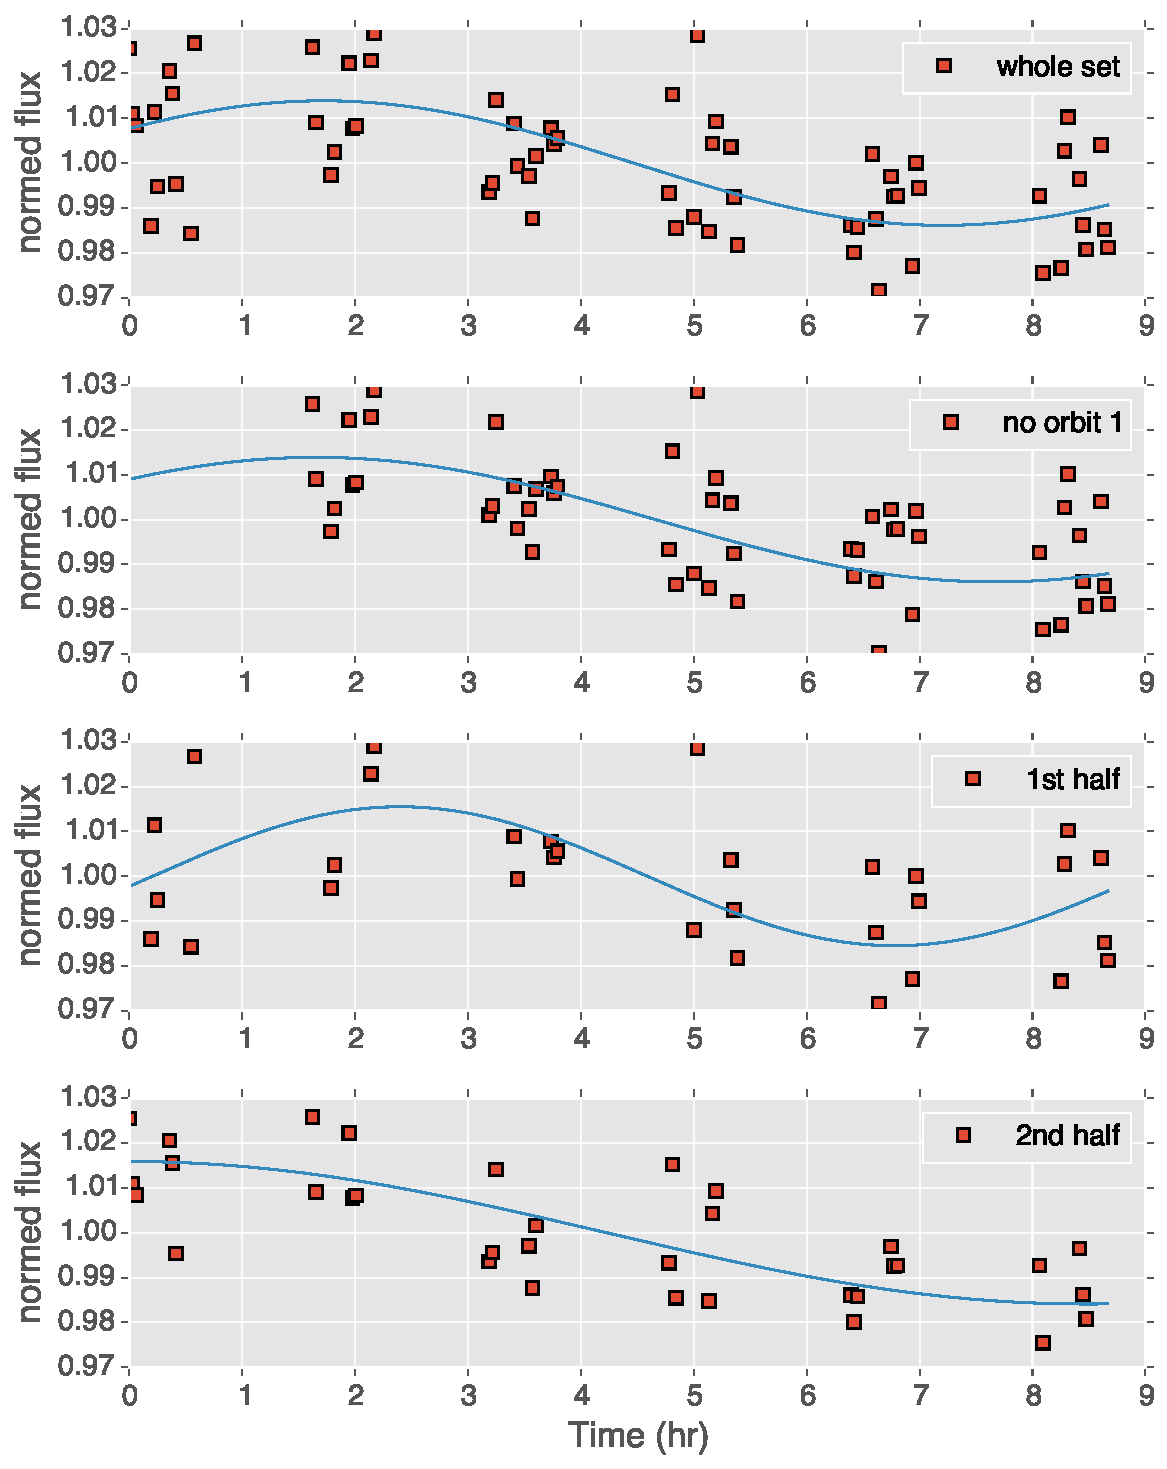
\includegraphics[width=0.48\textwidth]{F125W_SplitDataSet}
    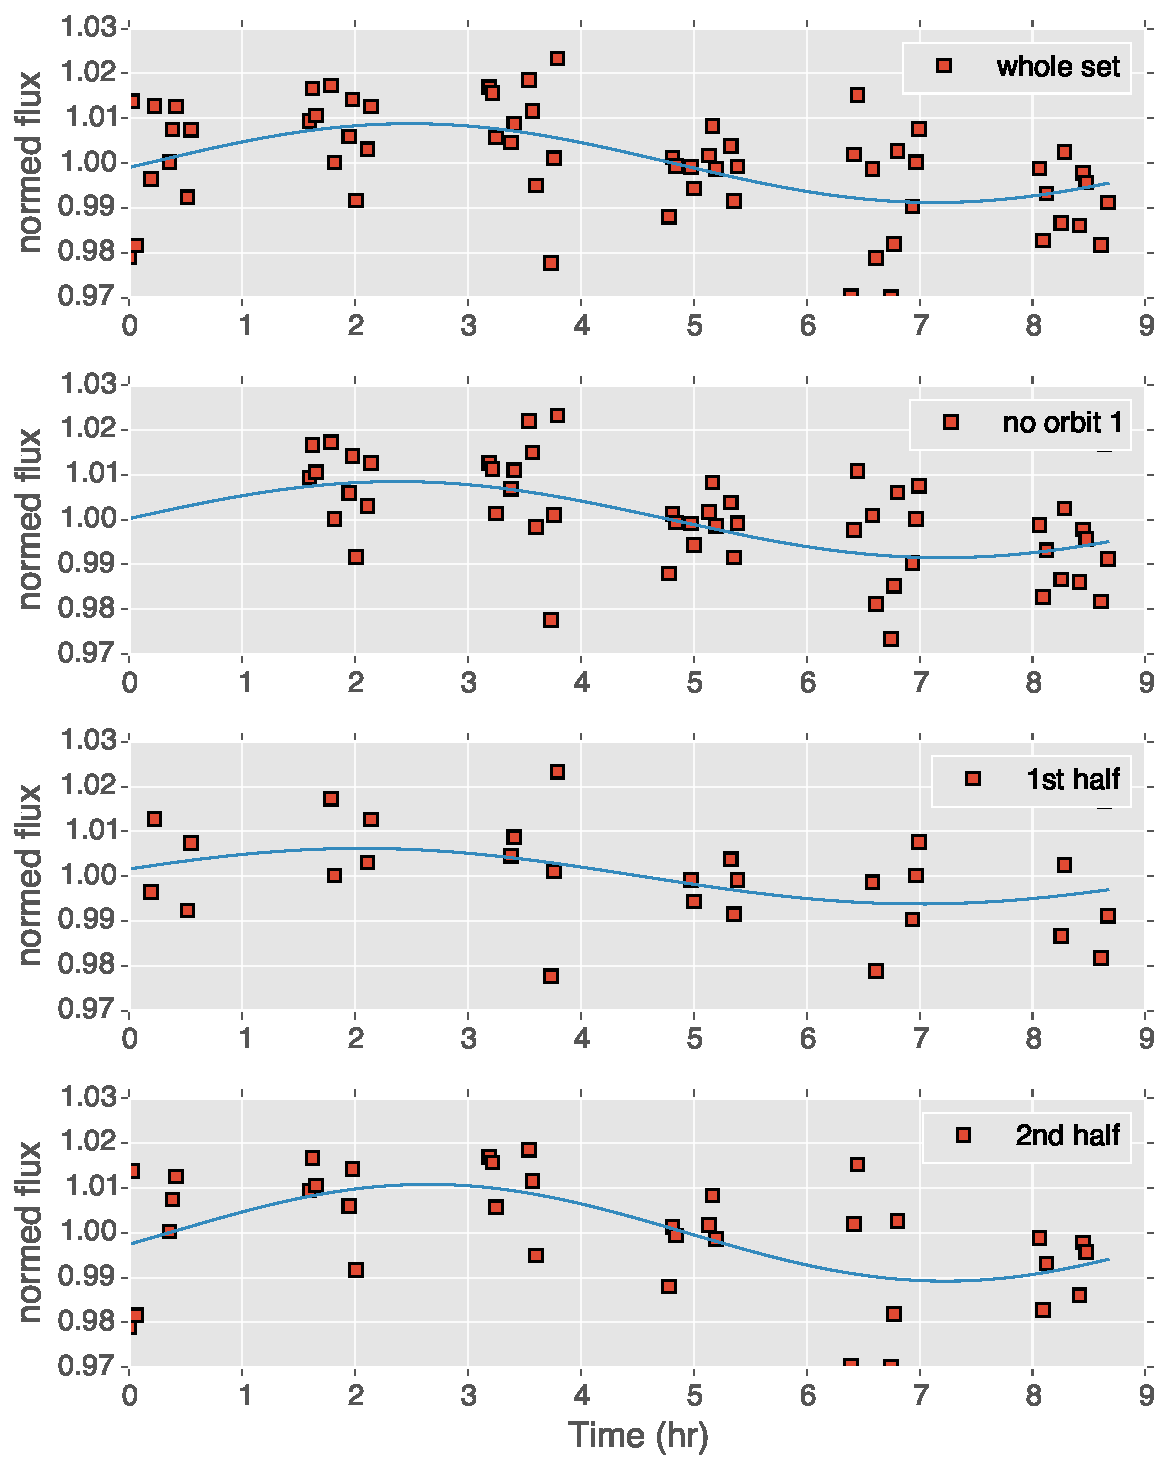
\includegraphics[width=0.48\textwidth]{F160W_SplitDataSet}
    \caption{phototmetry and fitted sine curves for different data
      set. The left panel is for F125W and the right is for F160W. The
    first row is the whole data set, the second is the fit with Orbit \# 1
  removed, the third is the fit for the first half and the forth is
  for the second half.}
    \label{fig:fit}
  \end{figure}


\embed{
3, My biggest (but not major) concern is the effect of flat fielding errors. I am not quite sure how to exclude their effect completely, perhaps Glenn has a good suggestion. Given that we don't really control the flat field errors, one test we should do is to introduce a flat field error and see what changes, if any, this introduces. I am thinking here on the following:
create an artificial flat error mask (AFEM) with uniformly distributed
noise with a mean value of 1.00 and a sigma of $\sim1\%$. Then
multiply all your frames with this AFEM right before you start the
actual reduction; and then compare the light curve emerging from your
AFEM reduction and the original one, including fitting a sine wave.}

\embed{
 I would think that a PSF model in which the residuals and the
 diffraction-limited (TinyTim) components are scaled together is more
 realistic than keeping the residuals fixed. Would you try scaling
 these together and see if the results are still the same?}

Actually by adding an artificial flat error mask or scaling the residual
together with the TinyTim PSFs together does not change the
photometric measurement too much. The F125W light curve measured as
original, with an AFEM, and with residual part scaling together with PSFs
are shown in Figure \ref{fig:compare}. The trends of the three light
curves are very similar. For measurement with an AFEM, the maximum
deviation of normalized photometry point from the original is around
0.005, which is $\sim50\%$ of the amplitude of the fitted sine
curve. For most of the data points, the deviation is below 0.002. For
the measurement with residual part scaling together with Tiny Tim
PSFs, the light curve is almost identical. The maximum difference
comparing to the original one is at $1\times10^{-4}$ level, which is
one order of magnitude smaller than the amplitude of the sine curve.
\begin{figure}[!h]
  \centering
  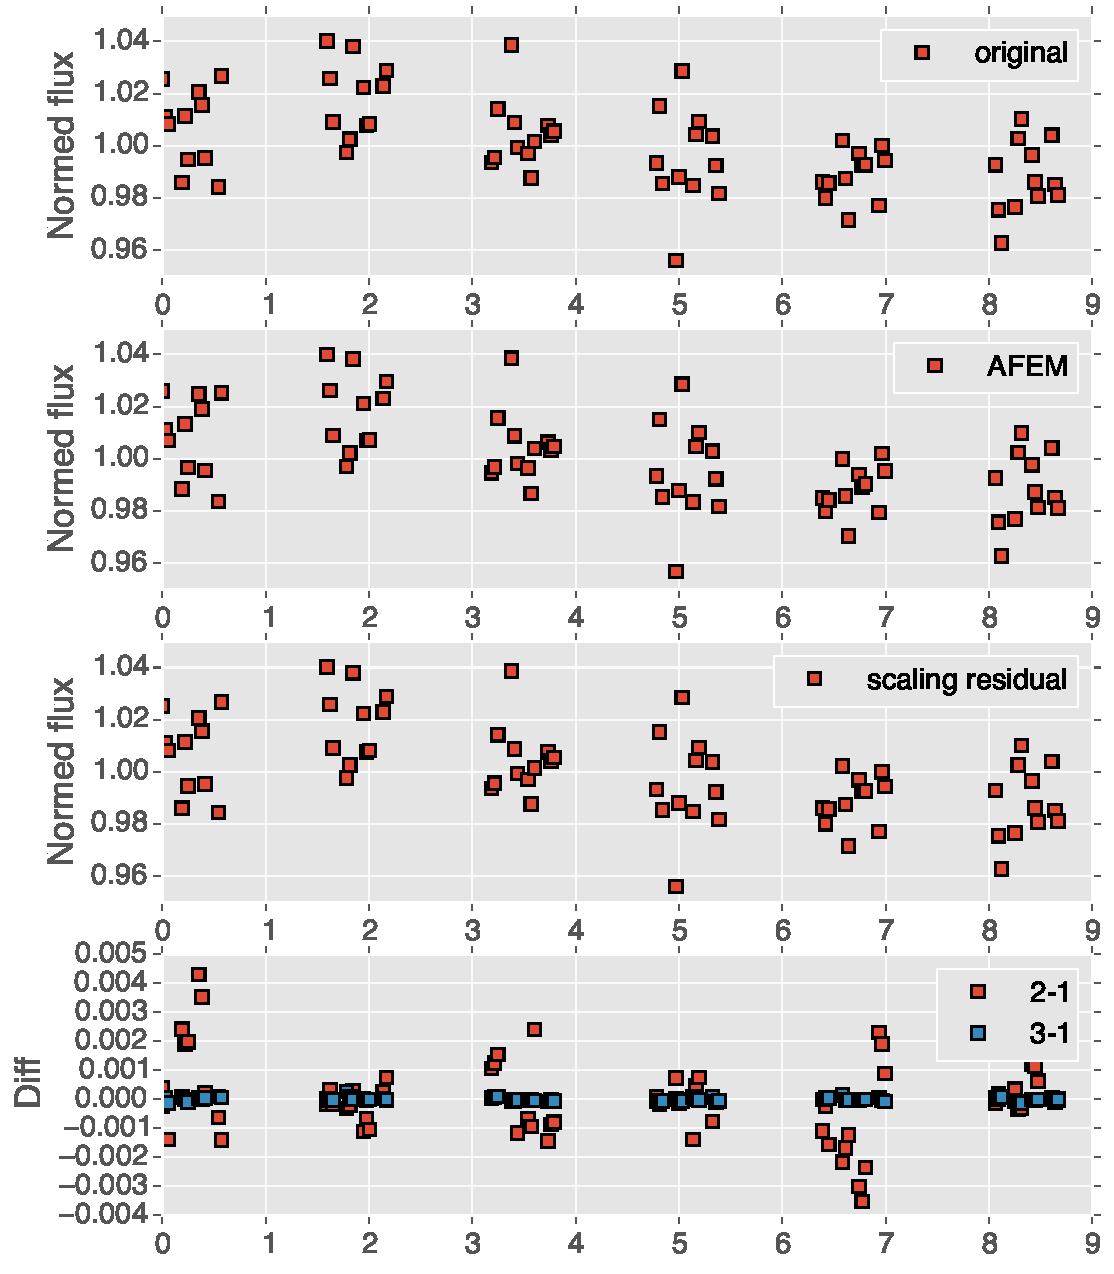
\includegraphics[height=0.5\textheight]{Diff}
  \caption{light curves of the original one (1st), the one measured with an
    AFEM applied (2nd), the one measured with residual part
    scaling together (3rd) and their difference. In the 4th panel, red
  points are the difference of the AFEM LC and the original LC, and
  blue points are the difference of the residual scaling LC and the
  original LC.}\label{fig:compare}
\end{figure}

\end{document}